\section{Turing machines}\label{sec:TMs}


% \begin{figure}[h!]
%     \centering
%     \begin{subfigure}[t]{0.45\textwidth}
%         \centering
%         \renewcommand{\arraystretch}{1.3} % Increase row height
%         \setlength{\tabcolsep}{12pt} % Increase column spacing
%         \vspace{10pt} % Adjust vertical alignment
%         \begin{tabular}{ccc}
%             \toprule
%                     & \textbf{0} & \textbf{1} \\
%             \midrule
%             \stateA & 1R\stateB  & 1L\stateC  \\
%             \stateB & 1R\stateC  & 1R\stateB  \\
%             \stateC & 1R\stateD  & 0L\stateE  \\
%             \stateD & 1L\stateA  & 1L\stateD  \\
%             \stateE & ---        & 0L\stateA  \\
%             \bottomrule
%         \end{tabular}
%         \caption{Transition table of the 5-state 2-symbol \BBfull winner. This machine was discovered by Marxen and Buntrock in 1989 \cite{Marxen_1990}.}
%         \label{table:bb5}

%         \vspace{10pt} % Adjust spacing
%         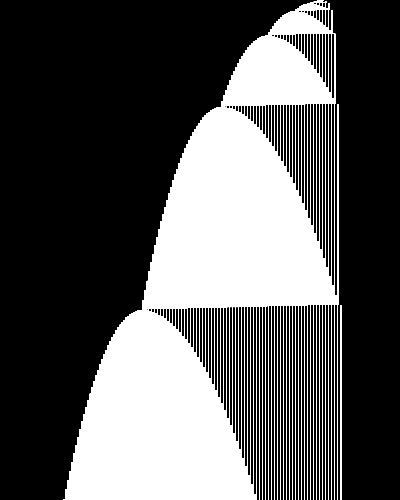
\includegraphics[width=0.7\linewidth]{figures/space-time-diagrams/bb5_20k.png} % Adjust the path as needed
%         \caption{20,000-step \textit{zoomed out} space-time diagram of the 5-state winner.}\label{fig:bb5-diagram-zoomout}
%     \end{subfigure}
%     \hfill
%     \begin{subfigure}[t]{0.45\textwidth}
%         \centering
%         \vspace{10pt} % Adjust vertical alignment
%         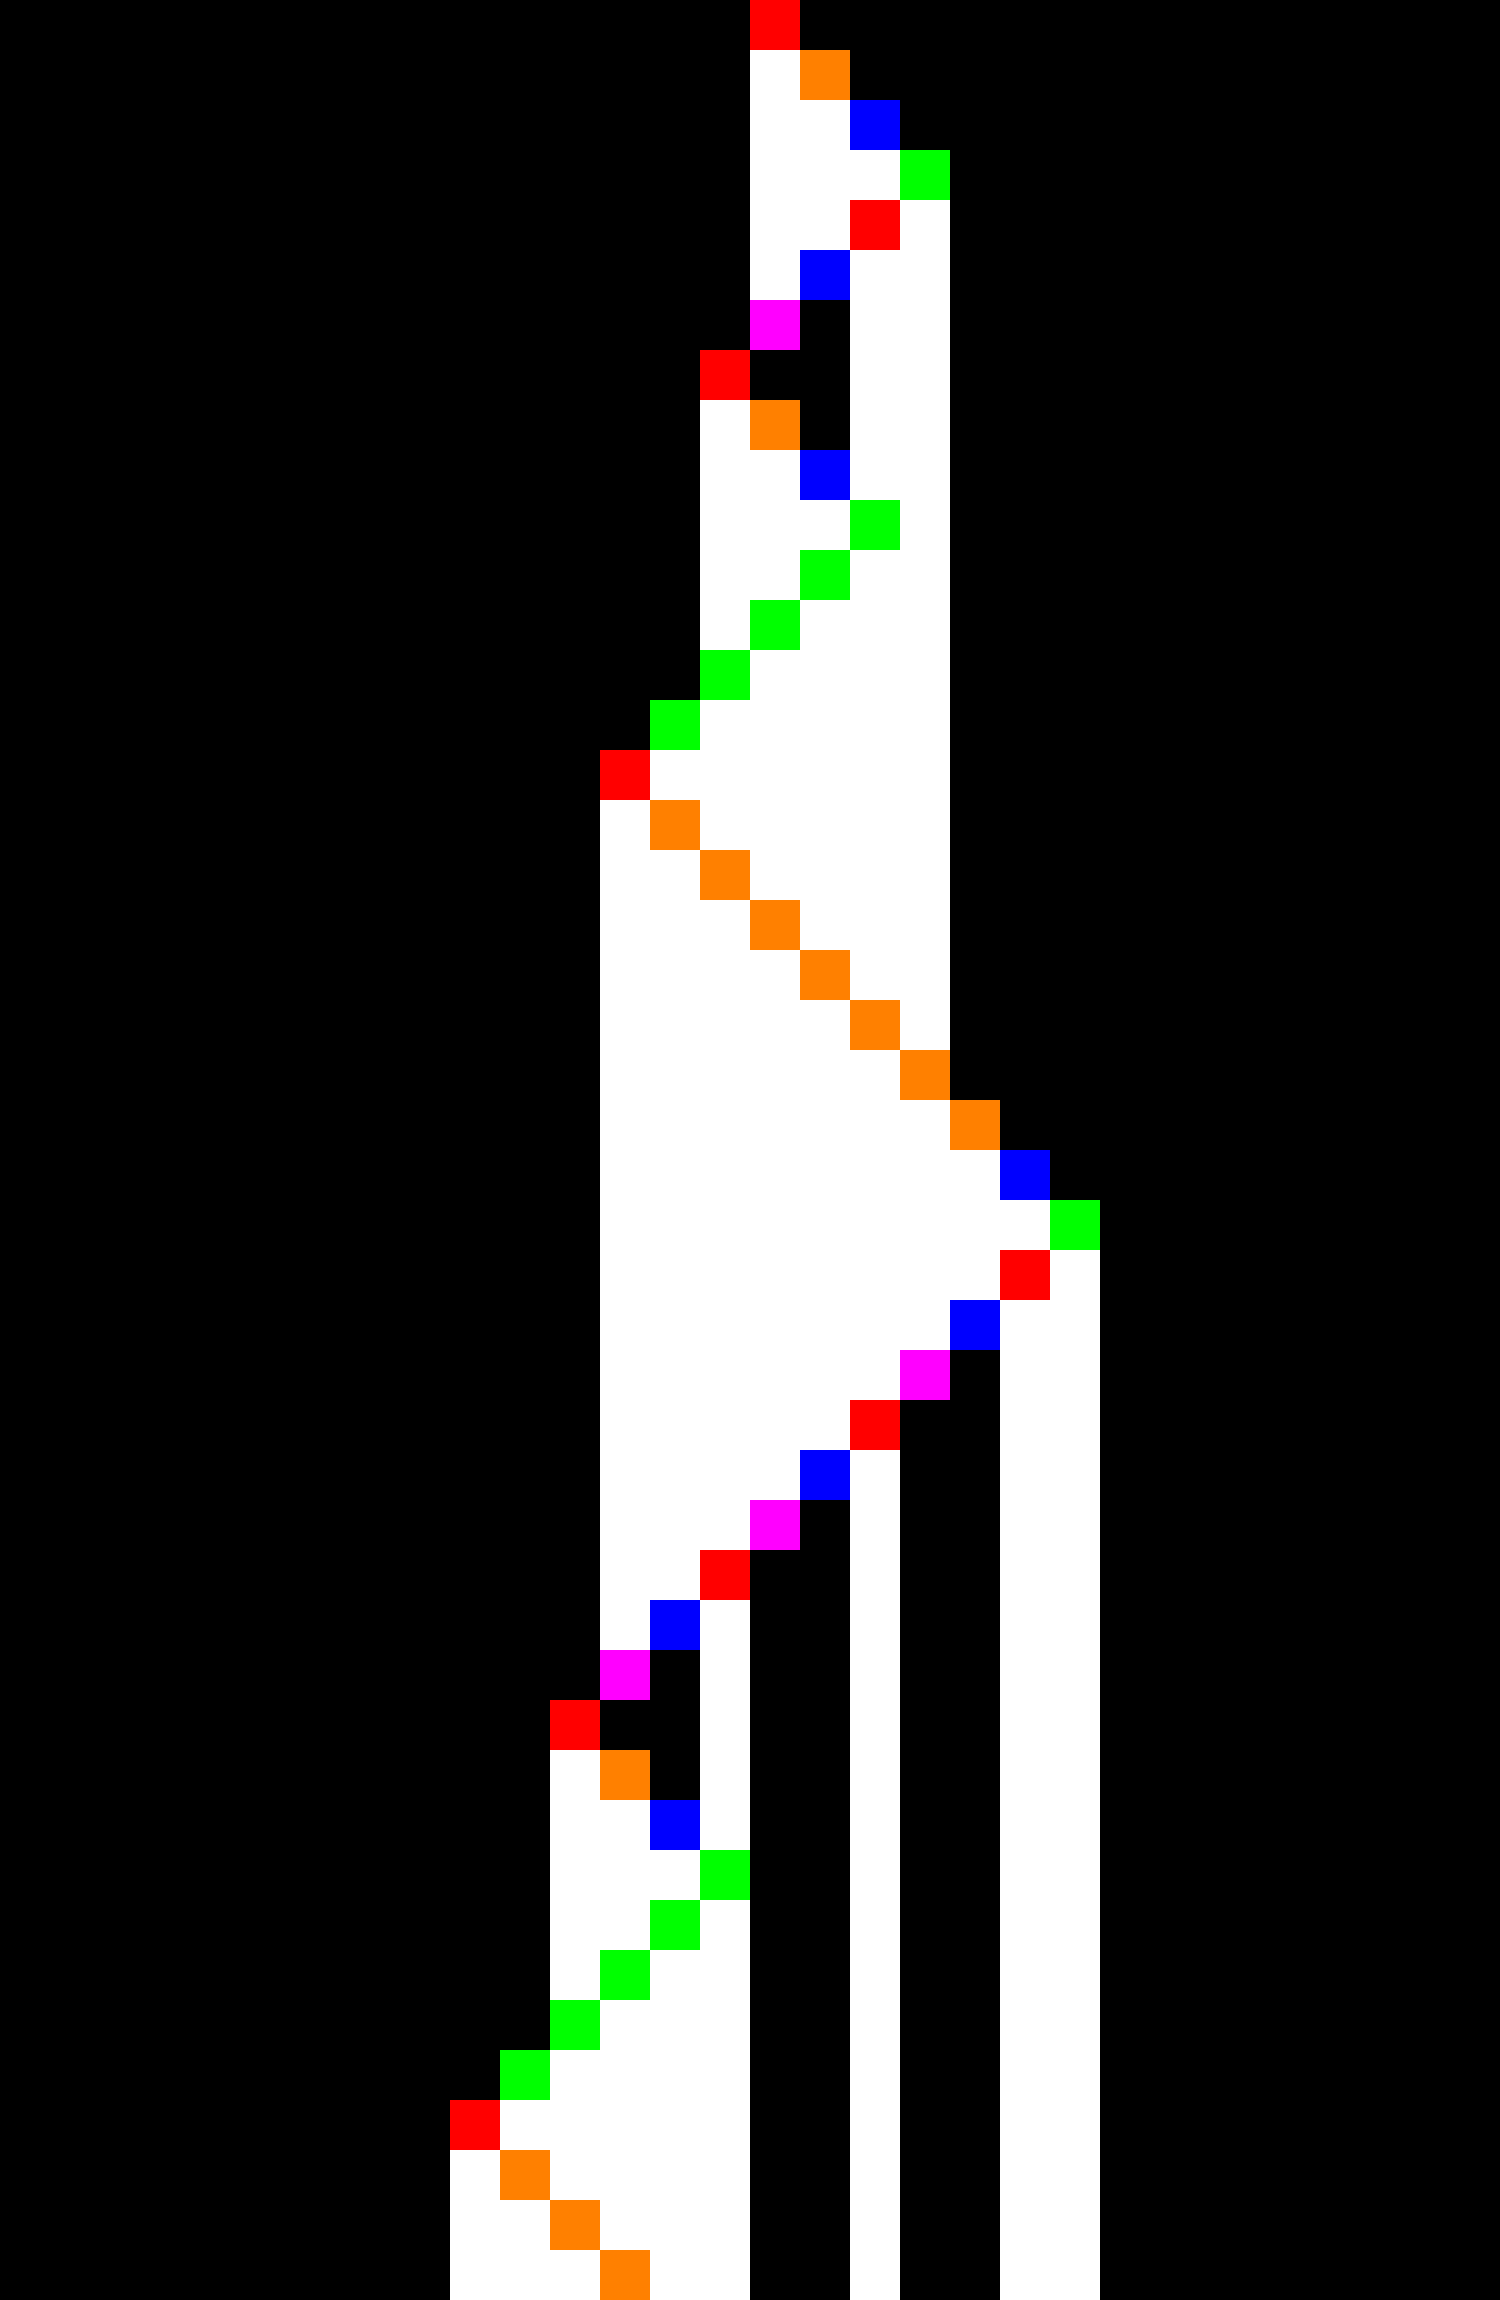
\includegraphics[width=0.7\linewidth]{figures/space-time-diagrams/bb5.pdf}
%         \caption{Space-time diagram of the first 45 steps of the 5-state winner.}
%         \label{fig:bb5-diagram}
%     \end{subfigure}
%     \caption{Transition table and space-time diagrams of the 5-state 2-symbol busy beaver winner, which halts after 47,176,870 steps.
%         \url{https://bbchallenge.org/1RB1LC_1RC1RB_1RD0LE_1LA1LD_---0LA}.}
%     \label{fig:bb5}
% \end{figure}

\begin{figure}[ht]
    \centering
    \renewcommand{\arraystretch}{1.3}
    \setlength{\tabcolsep}{6pt}

    \begin{subfigure}[b]{0.28\textwidth}
        \centering
        \begin{tabular}{ccc}
            \toprule
                    & \textbf{0} & \textbf{1} \\
            \midrule
            \stateA & 1R\stateB  & 1L\stateC  \\
            \stateB & 1R\stateC  & 1R\stateB  \\
            \stateC & 1R\stateD  & 0L\stateE  \\
            \stateD & 1L\stateA  & 1L\stateD  \\
            \stateE & ---        & 0L\stateA  \\
            \bottomrule
        \end{tabular}
        \caption{5-state 2-symbol \BBfull winner. This machine was discovered by Marxen and Buntrock in 1989 \cite{Marxen_1990}.}
        \label{table:bb5}
    \end{subfigure}
    \hfill
    \begin{subfigure}[b]{0.3\textwidth}
        \centering
        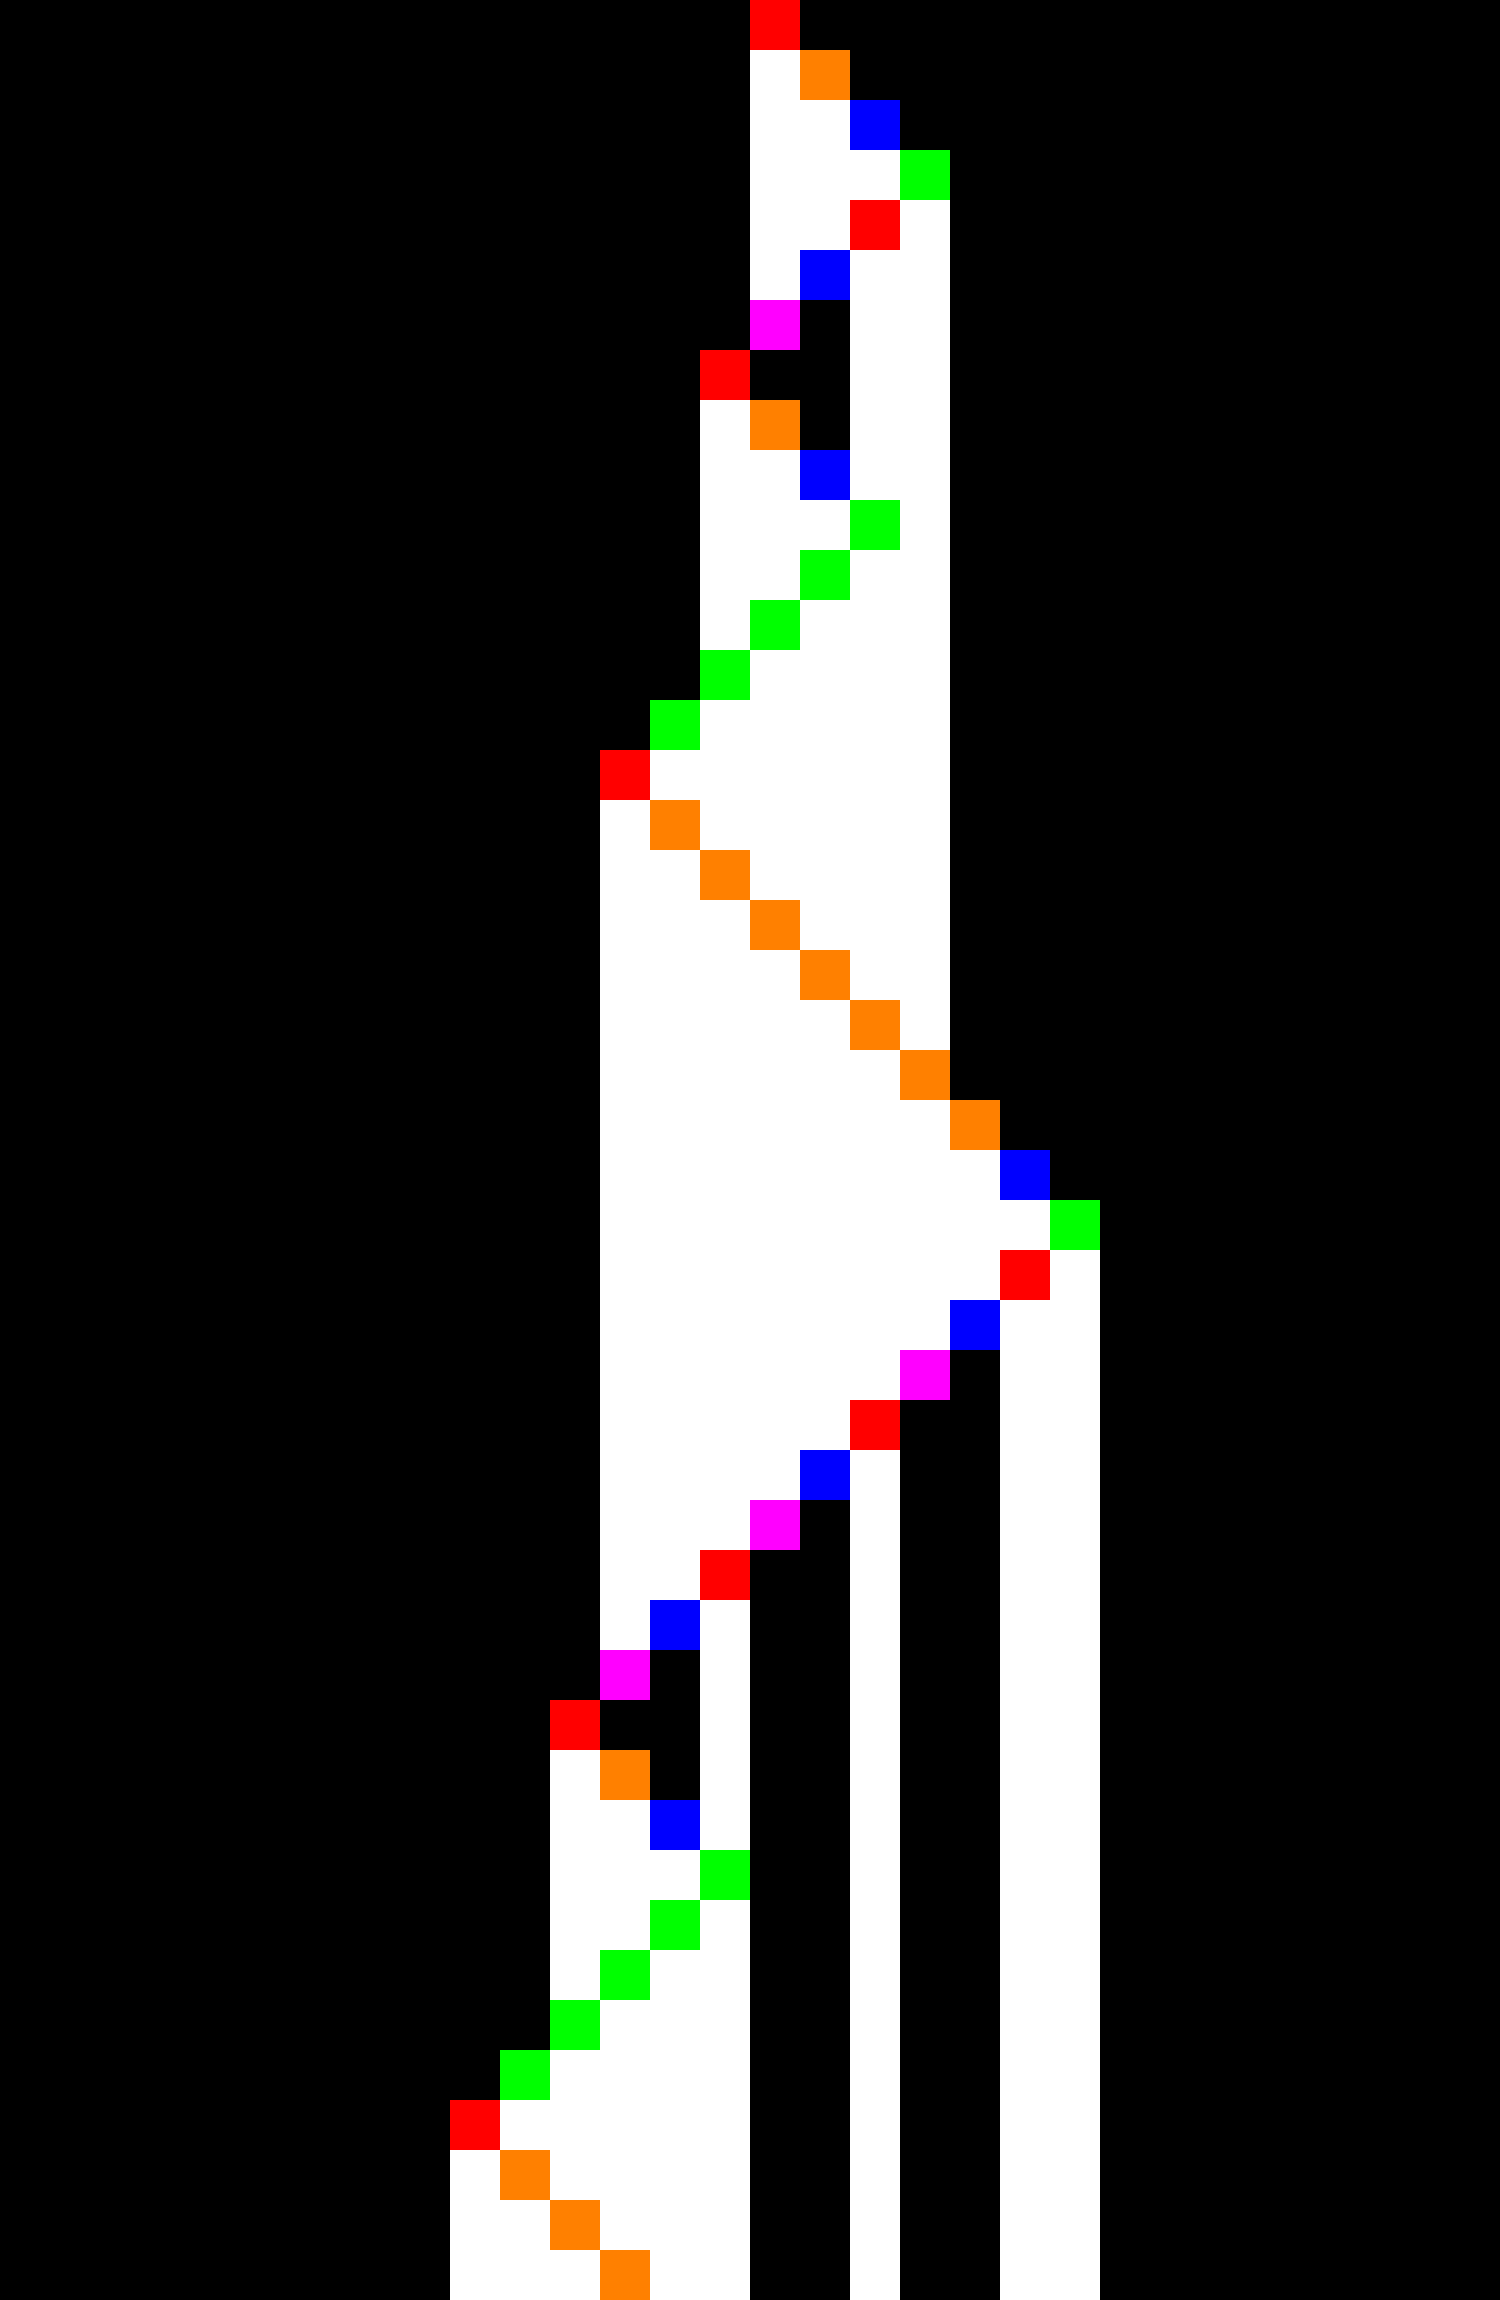
\includegraphics[width=0.87\linewidth]{figures/space-time-diagrams/bb5.pdf}
        \caption{Space-time diagram of the first 45 steps of the 5-state winner.}
        \label{fig:bb5-diagram}
    \end{subfigure}
    \hfill
    \begin{subfigure}[b]{0.3\textwidth}
        \centering
        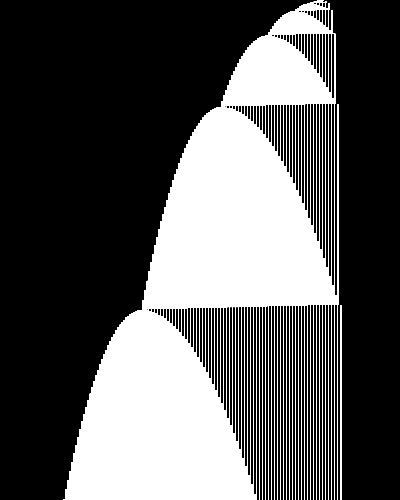
\includegraphics[width=\linewidth]{figures/space-time-diagrams/bb5_20k.png}
        \caption{20,000-step \textit{zoomed-out} space-time diagram of the 5-state winner.}\label{fig:bb5-diagram-zoomout}
    \end{subfigure}

    \caption{Transition table and space-time diagrams of the 5-state 2-symbol busy beaver winner, which halts after 47,176,870 steps.
        \url{https://bbchallenge.org/1RB1LC_1RC1RB_1RD0LE_1LA1LD_---0LA}.}\label{fig:bb5win}
\end{figure}






We consider Turing machines that use a single, discrete, bi-infinite tape -- \ie the tape can be thought of a function $t: \mathbb{Z} \to \alphabet$ with $\alphabet$ the alphabet of symbols used by the machine. Machine transitions are either undefined (the machine halts if it ever reaches an undefined transition) or given by (i) a symbol of $\alphabet$ to write (ii) a direction to move (right or left) and (iii) a state to go to -- \ie the transition table of a Turing machine is a partially defined function $\delta: \text{States} \times \alphabet \to \alphabet \times \{\text{L},\text{R}\} \times \text{States}$. Figure~\ref{fig:bb5win}(a) gives the transition table of the 5-state 2-symbol \BBfull winner. The machine halts after 47,176,870 steps (starting from all-0 tape) when it reads a \szero in state \stateE (undefined transition). Allowing for undefined transitions is a small, consequenceless but useful (see Section~\ref{sec:enum}), deviation from \rado's original setup.

In the \BBfull context, machines are always executed from the all-0 tape and starting in state \stateA. Execution goes as follows: at each step, the machine which is in state $s$ looks at which symbol $\sigma$ is present on the tape cell the head is currently on and then, if defined, executes the instruction given by its transition table, \eg $\delta(s, \sigma) = 0\text{L}\text{\stateE}$ means that the machine will write a \szero, move the cell on the left of the current one and switch to state \stateE. If $\delta(s, \sigma)$ is not defined, the machine halts.



A \textit{configuration} (also known as \textit{execution state}) of a Turing machine is defined by the 3-tuple: (i) state (ii) position of the head on the tape (iii) content of the memory tape. As mentioned above, here, \textit{the initial configuration} of a machine is always (i) state is A, i.e. the first state to appear in the machine's description (ii) head's position is 0 (iii) the initial tape is all-0 -- i.e. each memory cell is containing 0. We write $c_1 \TMstep_\mathcal{M} c_2$ if a configuration $c_2$ is obtained from $c_1$ in one computation step of machine $\mathcal{M}$. We omit $\mathcal{M}$ if it is clear from context. We let $c_1 \TMstep^s c_2$ denote a sequence of $s$ computation steps, and let $c_1 \TMstep^* c_2$ denote zero or more computation steps. % exact same wording as in https://dna.hamilton.ie/assets/dw/NearyWoodsFCT09.pdf
We write $c_1 \TMstep \bot$ if the machine halts after executing one computation step from configuration $c_1$. Halting happens when an undefined machine transition is met i.e. no instruction is given for when the machine is in the state, tape position and tape corresponding to configuration $c_1$.

% When discussing concrete configurations, we write
% $0^\infty\; s_1\; \cdots\; s_{k-1}\; [s_k]_q\; s_{k+1}\; \cdots\; s_n\; 0^\infty$
% to mean the configuration where the machine is in state $q$, with the head
% positioned on the symbol $s_k$, and the tape both starts and end by an infinite sequence of 0s, represented $0^\infty$. Thus, the initial configuration of the machine
% can be written as $0^\infty\; [0]_A\; 0^\infty$.

% \paragraph*{Directional Turing machines.} We will sometimes prefer to think of the tape head as being between
% symbols. Thus, we write $l \lhead{q} r$, with $l,r\in\{0,1\}^*$ to mean that the head is at the rightmost symbol
% of $l$, and $l \rhead{q} r$ to mean that the head is at the leftmost symbol of $r$.
% For example, $0^\infty\; [1]_A\; 0^\infty$ can be written as
% $0^\infty\; 1 \lhead A 0^\infty$ or $0^\infty \rhead A 1\; 0^\infty$.


\paragraph*{Space-time diagrams.} We use space-time diagrams to give a visual representation of the behavior of a given machine. The space-time diagram of machine $\mathcal{M}$ is an image where the $i^\text{th}$ row of the image gives:
\begin{enumerate}
    \item The content of the tape after $i$ steps (for 2-symbol machines, black is 0 and white is 1, while for $n$ symbols, black is 0, white is symbol $n-1$ and linear gray-scaling is used in between).
    \item The position of the head is colored to give state information using the following colours for 5-state machines: \textcolor{colorA}{A},  \textcolor{colorB}{B},  \textcolor{colorC}{C},  \textcolor{colorD}{D},  \textcolor{colorE}{E} (you have to look at the row above to deduce what symbol is the head reading, unless it is the initial row, where a \szero is read).
\end{enumerate}

Figure~\ref{fig:bb5win}(b) gives a 45-step space-time diagram for the 5-state 2-symbol \BBfull winner. We often use \textit{zoomed-out} space-time diagrams without state-coloring information, such as Figure~\ref{fig:bb5win}(c) which gives the 20,000 first steps of the 5-state 2-symbol \BBfull winner.


\paragraph*{Turing machine format.} We often communicate Turing machines using the following linear format: \\ \texttt{1RB1LC\_1RC1RB\_1RD0LE\_1LA1LD\_---0LA} represents the transition table of Figure~\ref{fig:bb5win}(a) where \texttt{\_} is used to separate states and transitions are given in read-symbol order. Note that, historically, the undefined transition reached by a halting machine was represented using \texttt{1RZ}, hence our format allows to use any letter outside of the state space to represent halting, \eg \texttt{1RB1LC\_1RC1RB\_1RD0LE\_1LA1LD\_1RZ0LA}. Multi-symbols machines are represented in the same way, \eg the 2-state 4-symbol \BBfull winner is \texttt{1RB2LA1RA1RA\_1LB1LA3RB---} (also given by \texttt{1RB2LA1RA1RA\_1LB1LA3RB1RZ}), see Figure~\ref{fig:bb2x4}.

This format can be used as URL for the \url{bbchallenge.org} website, \eg \url{https://bbchallenge.org/1RB1LC\_1RC1RB\_1RD0LE\_1LA1LD\_1RZ0LA} will display the transition table, space-time diagrams and known information about the machine.

\begin{figure}[ht]
    \centering
    \renewcommand{\arraystretch}{1.3}
    \setlength{\tabcolsep}{6pt}

    \begin{subfigure}[b]{0.3\textwidth}
        \centering
        \begin{tabular}{ccccc}
            \toprule
                    & \textbf{0} & \textbf{1} & \textbf{2} & \textbf{3} \\
            \midrule
            \stateA & 1R\stateB  & 2L\stateA  & 1R\stateA  & 1R\stateA  \\
            \stateB & 1L\stateB  & 1L\stateA  & 3R\stateB  & ---        \\
            \bottomrule
        \end{tabular}
        \caption{Transition table of the 2-state 4-symbol \BBfull winner found by Ligocki and Ligocki in 2005 \cite{PMichel_website}.}
        \label{table:bb2x4}
    \end{subfigure}
    \hfill
    \begin{subfigure}[b]{0.3\textwidth}
        \centering
        
\includegraphics[width=0.87\linewidth]{figures/space-time-diagrams/bb2x4.pdf}
        \caption{Space-time diagram of the first 45 steps of the 2-state 4-symbol winner.}
        \label{fig:bb2x4-diagram}
    \end{subfigure}
    \hfill

    \begin{subfigure}[b]{0.3\textwidth}
        \centering
        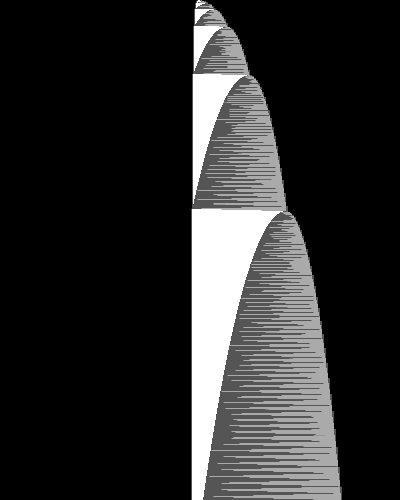
\includegraphics[width=0.5\linewidth]{figures/space-time-diagrams/bb2x4_20k.png} % Adjust the path as needed
        \caption{20,000-step \textit{zoomed out} space-time diagram of the 2-state 4-symbol winner.}\label{fig:bb2x4-diagram-zoomout}
    \end{subfigure}
    \caption{Transition table and space-time diagrams of the 2-state 4-symbol \BBfull winner, which halts after $\BBTxF$ steps.
        \url{https://bbchallenge.org/https://bbchallenge.org/1RB2LA1RA1RA_1LB1LA3RB---}.}
    \label{fig:bb2x4}
\end{figure}

